\iflanguage{ngerman}
{\chapter{Verwandte Arbeiten}}
{\chapter{Related Work}}
\label{sec:related}

The usefulness of smart contracts has been a focus of recent study, and numerous methods have been put out to improve it. We are attempting one method in which we employ Jason \ac{BDI} agents, which enables the construction of intelligent, autonomous agents that can interact with other agents to fulfill their objectives and put them in a supply chain. With the help of this strategy, supply chain roles like manufacturers have been given the ability to combine complicated decision-making and store their interactions in a blockchain network.

\vspace{.5cm}

The pertinent research in the field of agent programming using smart contracts will be covered in this part. These studies highlight the need for greater research in this area and imply that Jason \ac{BDI} agents can enhance the functionality of smart contracts when employed in a supply chain. The associated papers' subjects were arranged to address the following literature research questions (LRQ): 
\begin{itemize}[label={}]
    \item \textbf{LRQ1.}\label{LRQ1.} How to build intelligent agents within \ac{MAS} using \ac{AOP} language while comparing it with \ac{OOP}? \\

    \item \textbf{LRQ2.}\label{LRQ2.} What are the frameworks available for creating agents using the \ac{BDI} model?\\
    
    \item \textbf{LRQ3.}\label{LRQ3.} How to include smart contracts into \ac{MAS} in order to store transactions on a blockchain?\\

    \item \textbf{LRQ4.}\label{LRQ4.} What is the purpose of conducting further study when considerable research has already been done on the decentralized execution of smart contracts using the agent model?

\end{itemize}

\section{Assimilating Agents and Agent-Oriented Programming}

To address \hyperref[LRQ1.]{\textbf{LRQ1}} about learning about \ac{AOP}, \ac{MAS}, and other concepts to explore with our thesis, the articles listed below assisted in gaining a comprehensive view of all of the topics and understanding them better.

\begin{itemize}[label={}]
\item \textbf{Paper Title: \textit{Exploring \ac{AOP} from an \ac{OOP} perspective}}\\

Researchers in agent-oriented programming have created several agent programming languages that successfully connect theory and practice. Unfortunately, despite these languages' popularity in their communities, the larger community of software engineers has not found them to be as intriguing. The need to bridge the cognitive gap that exists between the notions behind standard languages and those underpinning \ac{AOP} is one of the key issues facing \ac{AOP} language developers. 
 
 \vspace{.5cm}
 
In this paper \cite{astra}, a conceptual mapping between \ac{OOP} and the AgentSpeak(L), family of \ac{AOP} languages was made; to create a linkage. This mapping examines how AgentSpeak(L) notions connect to \ac{OOP} principles and the concurrent programming concept of threads. After that, they used the study of this mapping to inform the creation of the \textbf{ASTRA} programming language.

 \vspace{.5cm}
 
\item \textbf{Paper Title: \textit{Jason}} for \ac{BDI} Agent Programming in AgentSpeak \\

This research \cite{jasonBDI} is based on the teaching provided as part of the CLIMA instructional VI program. The purpose of the lesson was to present a broad overview of the capability provided by Jason, a \ac{MAS} development platform based on an interpreter for an upgraded version of AgentSpeak. The \ac{BDI} architecture is the most well-known and thoroughly investigated architecture for cognitive agents, and AgentSpeak is a sophisticated, logic-based programming language inspired by the \ac{BDI} design.

\vspace{.5cm}

The study also highlights how agent-based technology has grown in popularity for a variety of reasons, including its suitability for the development of a wide range of applications, such as air traffic control, autonomous spacecraft management, healthcare, and industrial system control, to name a few. These are unquestionably application areas where dependable systems are required. The fact that formal verification approaches developed particularly for \ac{MAS} are also attracting a lot of academic attention and are expected to significantly influence agent technology adoption.

\vspace{.5cm}

\item \textbf{Paper Title: \textit{A Multi-agent System for Optimizing Urban Traffic}}\\

This article \cite{traffmulti} presents the creation of a hierarchical multi-agent framework for controlling an urban traffic system, which is made up of numerous locally running agents, each representing a traffic system intersection. Two traffic scenarios are studied to evaluate the operation of the proposed urban traffic multi-agent system. The multi-agent system efficiently controlled the network's progressive congestion in both circumstances (traffic accidents and morning rush hour).

\vspace{.5cm}

\item \textbf{Paper Title: \textit{Decision Making in Multiagent Systems: A Survey}} \\

In this study \cite{decision}, the researchers look at the most recent work on cooperative MAS decision-making models, such as Markov decision processes, game theory, swarm intelligence, and graph theoretic models. Reinforcement learning, dynamic programming, evolutionary computing, and neural networks are examples of algorithms that produce optimum and suboptimal policies.

\vspace{.5cm}

The researchers also talk about how these models may be used in robotics, wireless sensor networks, cognitive radio networks, intelligent transportation systems, and smart electric grids. Furthermore, the researchers define key terms in the field and discuss remaining challenges such as incorporating big data advances into decision making, developing autonomous, scalable, and computationally efficient algorithms, tackling more complex tasks, and developing standardized evaluation metrics.

\vspace{.5cm}

\item \textbf{Paper Title: \textit{Agent-Oriented Supply-Chain Management}} \\

In order to build an agent-oriented software architecture for controlling the supply chain at the tactical and operational levels, this paper \cite{agSupch} examines problems and offers solutions. The method is based on the employment of an agent building shell, which offers assured, reusable, and generic components. It sees the supply chain as being made up of a group of intelligent software agents, each of which is in charge of one or more supply chain activities. 

\vspace{.5cm}

These agents collaborate with one another to plan and carry out their tasks and provide services for communicative-act-based communication, conversational coordination, role-based organization modeling, and other things. They attempted to demonstrate two nontrivial agent-based supply-chain designs using these elements that might allow intricate cooperative work and the control of disruption brought on by stochastic occurrences in the supply chain.

\vspace{.5cm}

The objective of developing models and methods that allow \ac{MAS} to do coordinated work in practical applications has been advanced by the research in a number of different ways. All the strategies are carried out by the agents, which causes several organized dialogues to occur amongst the agents. These concepts have been supported by the development of a useful, application-neutral coordination language that offers tools for describing coordination-enhanced plans as well as the interpreter supporting their execution. The researcher of the study has tested the coordination language and the shell on a number of issues, including supply chain coordination initiatives carried out in collaboration with industry. Despite the fact that the number of solutions they built and the number of users of our system are both limited, the evidence they have so far shows that their methodology is promising in terms of the naturalness of the coordination model, the effectiveness of the representation and power, and the usability of the provided programming tools.
\end{itemize}

\vspace{.5cm}

There is Jason framework that we are about to use in order to create agents which facilitates reasoning about beliefs, desires, and intentions, as well as agent communication. However there are other frameworks available that support the \ac{BDI} paradigm and \ac{MAS}. \hyperref[LRQ2.]{\textbf{LRQ2}} led us to these research articles presented below to understand better.

\newpage

\begin{itemize}[label={}]

\item \textbf{Paper Title: \textit{Languages for Programming \ac{BDI}-style Agents: an Overview}}\\

In this paper \cite{9lang}, nine languages and systems are reviewed and compared namely PRS, dMARS, JACK, JAM, Jadex, AgentSpeak(L), 3APL, Dribble, and Coo-\ac{BDI}. There are additional links to other systems and languages based on the \ac{BDI} concept, as well as surveys dealing with relevant themes.

\vspace{.5cm}

\item \textbf{Paper Title: \textit{A Review of Agent Platforms}}\\

The goal of the paper \cite{review} is to give information on various frameworks and conduct an in-depth analysis. It offers details on active projects, projects whose status is unknown in relation to certain platform types, such as general-purpose, special-purpose, modeling-simulation platforms, and platforms that are no longer being developed. It also shows \ac{MAS} development techniques.

\vspace{.5cm}

Table \ref{BDI model frameworks} in Chapter 6 has been likewise structured with the assistance of this research.

\vspace{.5cm}

\item \textbf{Paper Title: \textit{Domain specific agent-oriented programming language based on the Xtext framework}} \\

One of the most reliable methods for creating distributed systems is the agent technology. A runtime environment that allows the execution of software agents is presented by the multi-agent middleware XJAF. The researchers suggest a domain-specific agent language called \textbf{ALAS}, whose major function is to facilitate the construction and execution of agents across heterogeneous platforms, in order to address the issue of incompatibility. According to the demands and needs of the agents, a metamodel and grammar of the ALAS language have been developed to describe the language's structure. The development of the compiler and the creation of Java executable code that can be run in XJAF are both covered in this paper \cite{xtext}.

\vspace{.5cm}

\item \textbf{Paper Title: \textit{A Survey of Agent Platforms}}\\

The article \cite{survey} provides an up-to-date comparative analysis of the most promising current agent platforms that can be deployed. It is built on universal comparison and assessment standards, offering classes to assist readers understand which agent platforms have roughly comparable qualities and which decisions should be made in which scenarios.

\vspace{.5cm}

In this article, the researchers offered a practical guideline recommendation for comparing and evaluating agent platforms, which is directly related to the scope of platform operation and the quality of each platform's given feature. This guidelines proposal is divided into five criterion categories: platform qualities, usability, operational abilities, pragmatics, and security management. Each of these categories has a number of subcriteria suggesting an in-depth assessment of each agent platform.

\newpage

\item \textbf{Paper Title: \textit{Multi-agent oriented programming with JaCaMo}}\\

The researchers presented a complete strategy for multi-agent oriented programming that combines the agent, environment, and organizational levels, giving a programming model that tries to connect relevant abstraction elements in an effective and synergistic way. To put the concept into reality, the researchers developed the JaCaMo platform, which integrates and expands current techniques and supporting technologies, particularly Jason (agent dimension), CArtAgO (environment dimension), and Moise (communication dimension) (organisation dimension).  In this paper \cite{Jacamo}, a case study and various applications were used to demonstrate the overall strategy.

\vspace{.5cm}

\item \textbf{Paper Title: \textit{Brahms: A multiagent modelling environment for simulating work processes and practices}}\\

The researchers suggest in this paper \cite{brahms} that the Brahms language is appropriate for researching many social and work practice issues of relevance to the organizational process modeling community. Their modeling work practice experience and findings imply that wider social problems may also be simulated. The Brahms modeling language provides significant advantages for researchers because, when compared to other tools like as Swarm, it allows for a more "natural" description of human behavior at the level of activities, reasoning, communication, contact with objects, and mobility in the world.

\vspace{.5cm}

Brahms, like other \ac{BDI} languages, is a declarative language, but it is distinct from the other \ac{BDI} languages in numerous ways:
Brahms is an activity-based language, whereas the majority of other \ac{BDI} languages are task-based. Brahms has a subsumption design, whereas most other \ac{BDI} languages employ a goal-based architecture; it supports environment modeling (geography), agent mobility in the environment, and so on; Finally, Brahms provides a distinct fact-state for modeling the world state outside of the agent's belief-set, whereas typical \ac{BDI}-languages only describe agents with an independent belief-state.

\vspace{.5cm}

\item \textbf{Paper Title: \textit{Jadex: A \ac{BDI}-Agent System Combining Middleware and Reasoning}}\\

This article \cite{jadex} describes a method for integrating an agent middleware with a reasoning engine in order to maximize the benefits of both strands. The reason for agent-oriented middleware was discussed, as well as an overview of the \ac{BDI} model, and the design and implementation of the Jadex \ac{BDI} engine as an extension to the widely used JADE agent platform. The Jadex system enables the creation of rational beings with goal-directed (rather than task-oriented) behavior. The Jadex agents are built using well-established software engineering approaches such as XML, Java, and OQL, allowing software professionals to swiftly capitalize on the possibilities of the mentalistic approach.

\newpage

\item \textbf{Paper Title: \textit{LightJason, a Highly Scalable and Concurrent Agent Framework: Overview and Application}}\\

The paper \cite{lightjason} provides an overview and use of LightJason, a highly scalable Java-based \ac{AOP} and simulation platform. The researchers describe the architectural elements of LightJason and demonstrate its applicability via the use of an example of a browser-based web application that implements a traffic serious game designed to instruct an interdisciplinary student team in \ac{MAS} and \ac{AOP}.

\vspace{.5cm}

The use-case model illustrates a highway traffic scenario that is used to teach \ac{MAS} and \ac{AOP} to students. Vehicles, road segments with speed restrictions, and traffic rule enforcement are all modeled as \ac{BDI} agents. The researchers focused on how LightJason supports integrating agent technology into cutting-edge browser-based web applications, which is difficult with existing agent frameworks, which are mostly stand-alone with "hard-wired" integrated development environments, runtime, graphical user interface, and source editor. These components are modular in LightJason, making the structure lightweight, versatile, and simple to incorporate.

\end{itemize}


\section{Linking Blockchain with Agents}

The principal objective was to include \ac{BCT} into \ac{MAS}, which is a very current and innovative subject that may be applied in a futuristic supply chain. Some researchers have already worked on it, which has given us some ideas on how to run smart contracts by the agents, created using Jason framework. The papers listed below are aligned to our work and can be read to have a stronger insight to answer the \hyperref[LRQ3.]{\textbf{LRQ3}} we posed in this chapter.

\begin{itemize}[label={}]

\item \textbf{Paper Title: \textit{From Agents to Blockchain: Stairway to Integration}} \\

The researchers who conducted this study attempted to throw some insight on the most recent integration efforts, mostly from a "agent-vs.-blockchain" perspective. They stressed the possibility of an alternate strategy, which they referred to as "agent-to-blockchain." Finally, they described the "agent-to-blockchain" approach along a pathway upgrading smart contracts towards complete agency, in both dimensions, after acknowledging the presence of two integration dimensions, a computational and an interactional one.

\vspace{.5cm}

In this paper \cite{ag2bc}, the researchers give a roadmap and emphasize the issues that still need to be addressed in order to comprehend the prospects, dimensions to consider, and several methods for merging agents with blockchain. They then discussed the case of Tenderfone \cite{tenGlab}, a custom blockchain that offers proactive smart contracts as the first step along the roadmap, equipping smart contracts with control flow encapsulation, reactivity to time, and asynchronous communication means, as both validation of their roadmap and a foundation for future development.

\vspace{.5cm}

\item \textbf{Paper Title: \textit{Decentralized Execution of Smart Contracts: Agent Model Perspective and Its Implications}}\\

After close scrutiny, the authors of the paper \cite{decentralized} concluded that users who are connected with a smart contract may deliberately try to influence the contract's execution in order to improve their own advantages. In order to address this issue and discuss the possibility of preventing users from manipulating smart contract execution by using game theory and agent based analysis, the authors of this paper propose an agent model as the underlying mechanism for contract execution over a network of decentralized nodes and public ledger.

\vspace{.5cm}

The authors of this paper created an agent-based framework to simulate the execution of smart contracts over a decentralized network of nodes and participants using blockchain and public ledger. Unlike the wias held belief that smart contract execution results can be trusted, the agent-based model of smart contract execution assumes that nodes may have the incentive to influence or lie about contract execution results in exchange for personal benefits or financial gains, even if they are not directly involved in a contract. It had been noted that users who are directly or indirectly involved in a smart contract may behave intelligently to influence the execution outcome of the smart contract. According to the agent-based approach, it might be possible to stop users from cheating when it comes to contract execution or lying about the outcome.

\vspace{.5cm}

It has also been demonstrated that it is realistic to prohibit users from lying about outcomes or manipulating contract execution results if penalties are applied during contract execution and the assumption is made that users are not totally confident in the rationality of other participants. Furthermore, it had been thought that studying irrationality will help us understand how users behave in a decentralized crypto-currency or smart contract system. An important outstanding challenge is the systematic study of irrationality in relation to the execution and consensus of smart contracts. If it is feasible to employ other mechanisms, such than a monetary penalty, to discourage users from lying about contract outcomes when it benefits them, that would be an intriguing open challenge raised in the paper.

\vspace{.5cm}

\item \textbf{Paper Title: \textit{MAS and Blockchain: Results from a Systematic Literature Review}} \\

The creation of intelligent distributed systems that manage sensitive data makes extensive use of the \ac{MAS} technology. The usage of \ac{BCT} for \ac{MAS}  is encouraged by current trends in order to promote accountability and trustworthy connections. The researchers explained that as most of these techniques have just recently begun to investigate the subject, it is important to build a research road map and identify any relevant scientific or technological hurdles.

\vspace{.5cm}

This paper\cite{literature} includes a thorough literature evaluation of trials using \ac{MAS} and \ac{BCT} as the first required step toward achieving this aim. The authors examined the reasons, presumptions, prerequisites, characteristics, and limits offered in the current state of the art in an effort to give a thorough review of their application fields. They also lay out their vision for how \ac{MAS} and \ac{BCT} may be coupled in various application situations while noting upcoming hurdles.

\vspace{.5cm}

\item \textbf{Paper Title: \textit{Self-Aware Smart Contracts with Legal Relevance}} \\

This paper \cite{sac} introduces a revolutionary, blockchain-agnostic paradigm for cross-organizational peer-to-peer cooperation. When new blockchain technology enabled smart contracts are paired with intelligent multi-agent systems, they provide so-called self-aware contracts, which offer a high degree of automation for such peer-to-peer partnerships.

\vspace{.5cm}

It was revealed that combining \ac{BDI} agents with the declarative SAC-Language results in self-aware contracts, where the former ensure that trustworthy information is routed into contract-based collaborations as a merged set. The researchers accomplished human manageability of the self-aware contract framework by offering a declarative smart-contract language that defines cross-organizational contract-collaborations, in addition to deploying agents that give a degree of artificial intelligence in a collaboration.
\end{itemize}

\vspace{.5cm}

Understanding how applications employing \ac{MAS} and smart contracts are deployed inside a supply chain is crucial to ascertain if smart contracts and agents can be used to build a fair and efficient dispute resolution procedure in a supply chain. 

\vspace{.5cm}

As mentioned in \hyperref[LRQ4.]{\textbf{LRQ4}}, some work has been done combining agents and blockchain, however we are conducting additional research in this area because the agents we are about to use are \ac{BDI} agents with Jason framework, which are a type of software agent that can make autonomous decisions based on its beliefs about the environment, desires or goals, and intentions to achieve those goals. We are attempting to integrate blockchain technology into a multi-agent environment created using Jason framework in which intelligent agents can communicate with one another.\ac{BDI} agents can assist with supply chain management by arranging the flow of commodities, monitoring inventory levels, and negotiating with suppliers and consumers. 


\begin{figure}[h]
\centering
  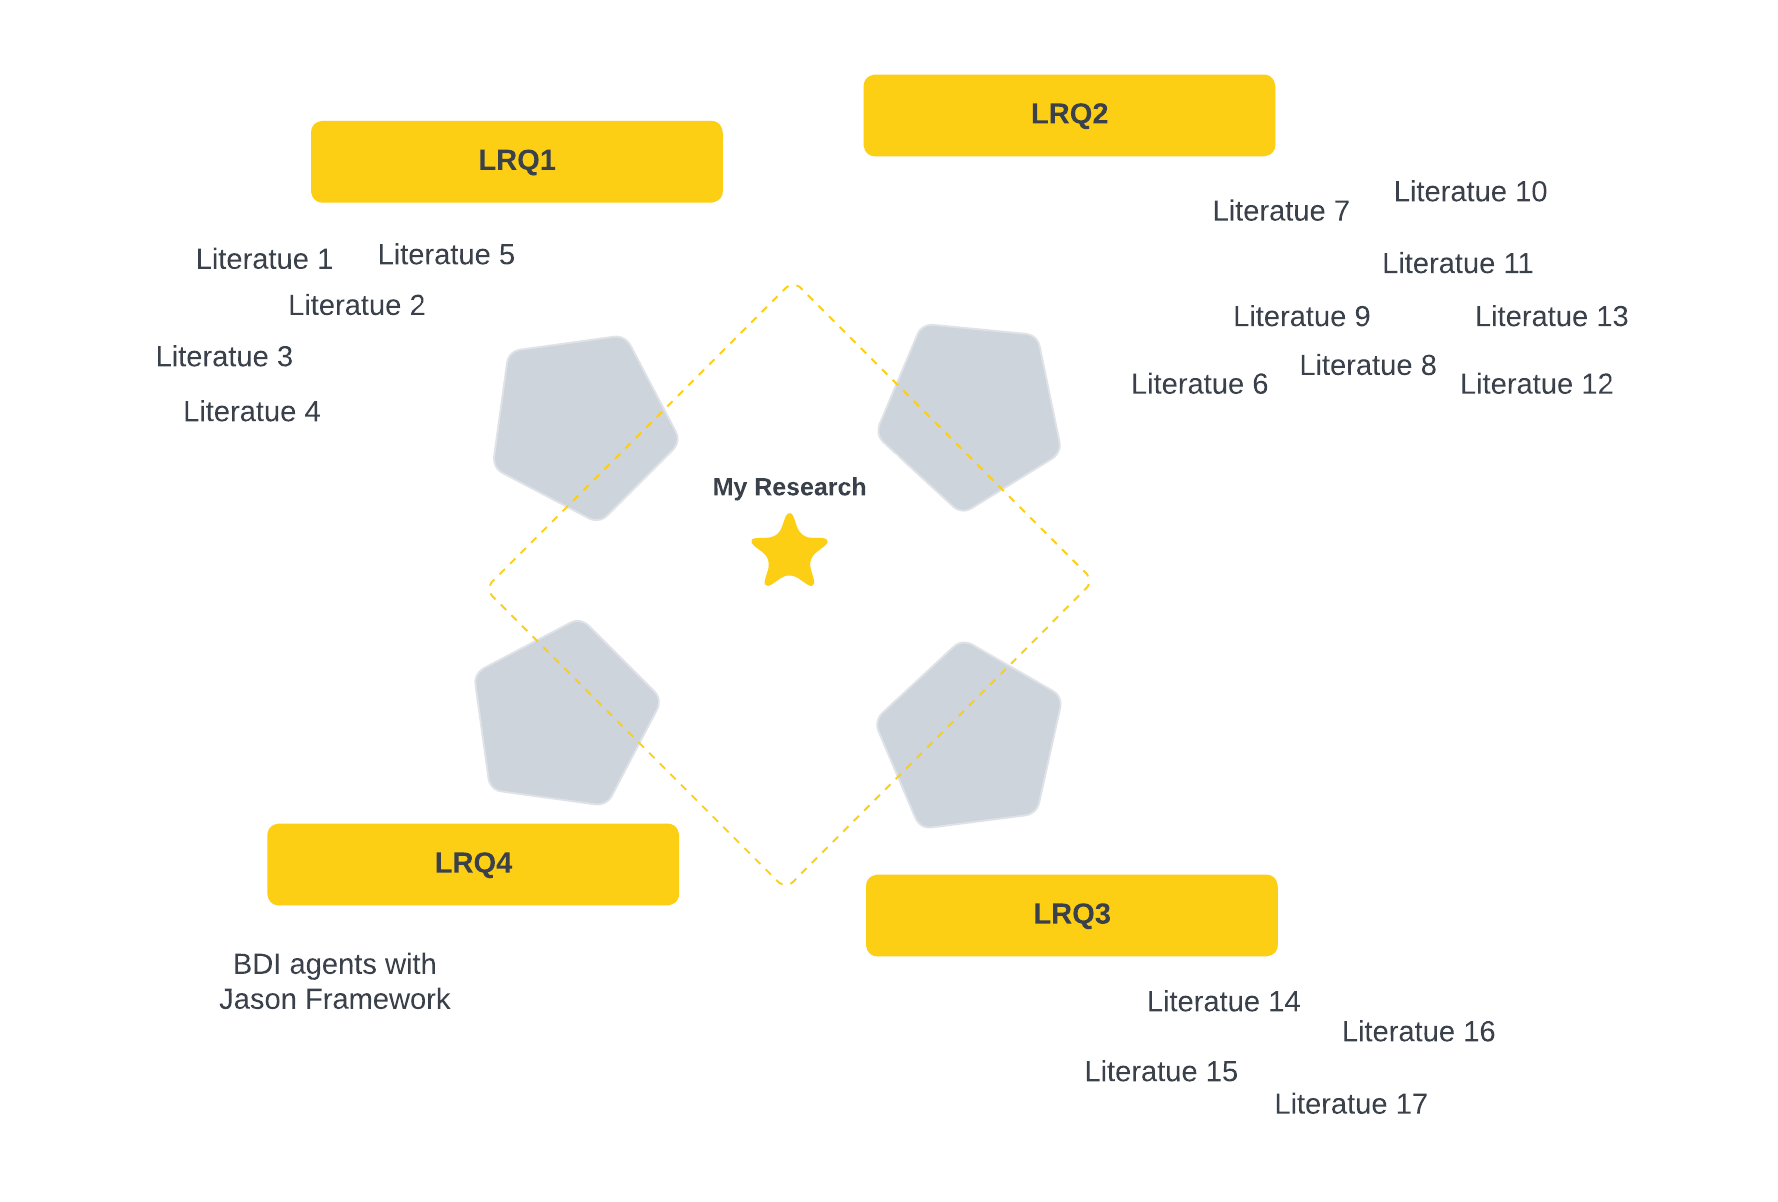
\includegraphics[width=10cm]{includes/figures/related work.png} 
  \caption{Literature Contribution}
  \label{related work}
\end{figure}

Figure \ref{related work} depicts a visual representation of the above-mentioned paper's contribution to our literature study and addressing the LRQs. The next chapters attempt to construct our own application utilizing solidity-written smart contracts with Jason \ac{BDI} agents to investigate if \ac{BDI} agents can enhance the collaboration, coordination and negotiation between supply chain members and if it can be used with smart contracts to manage unforeseen events and contingencies in supply chain.